\vspace{+0.4cm}
\section*{Speelbord}
\label{item:speelbord}

\begin{comment}
\begin{center}
  \makebox[\textwidth]{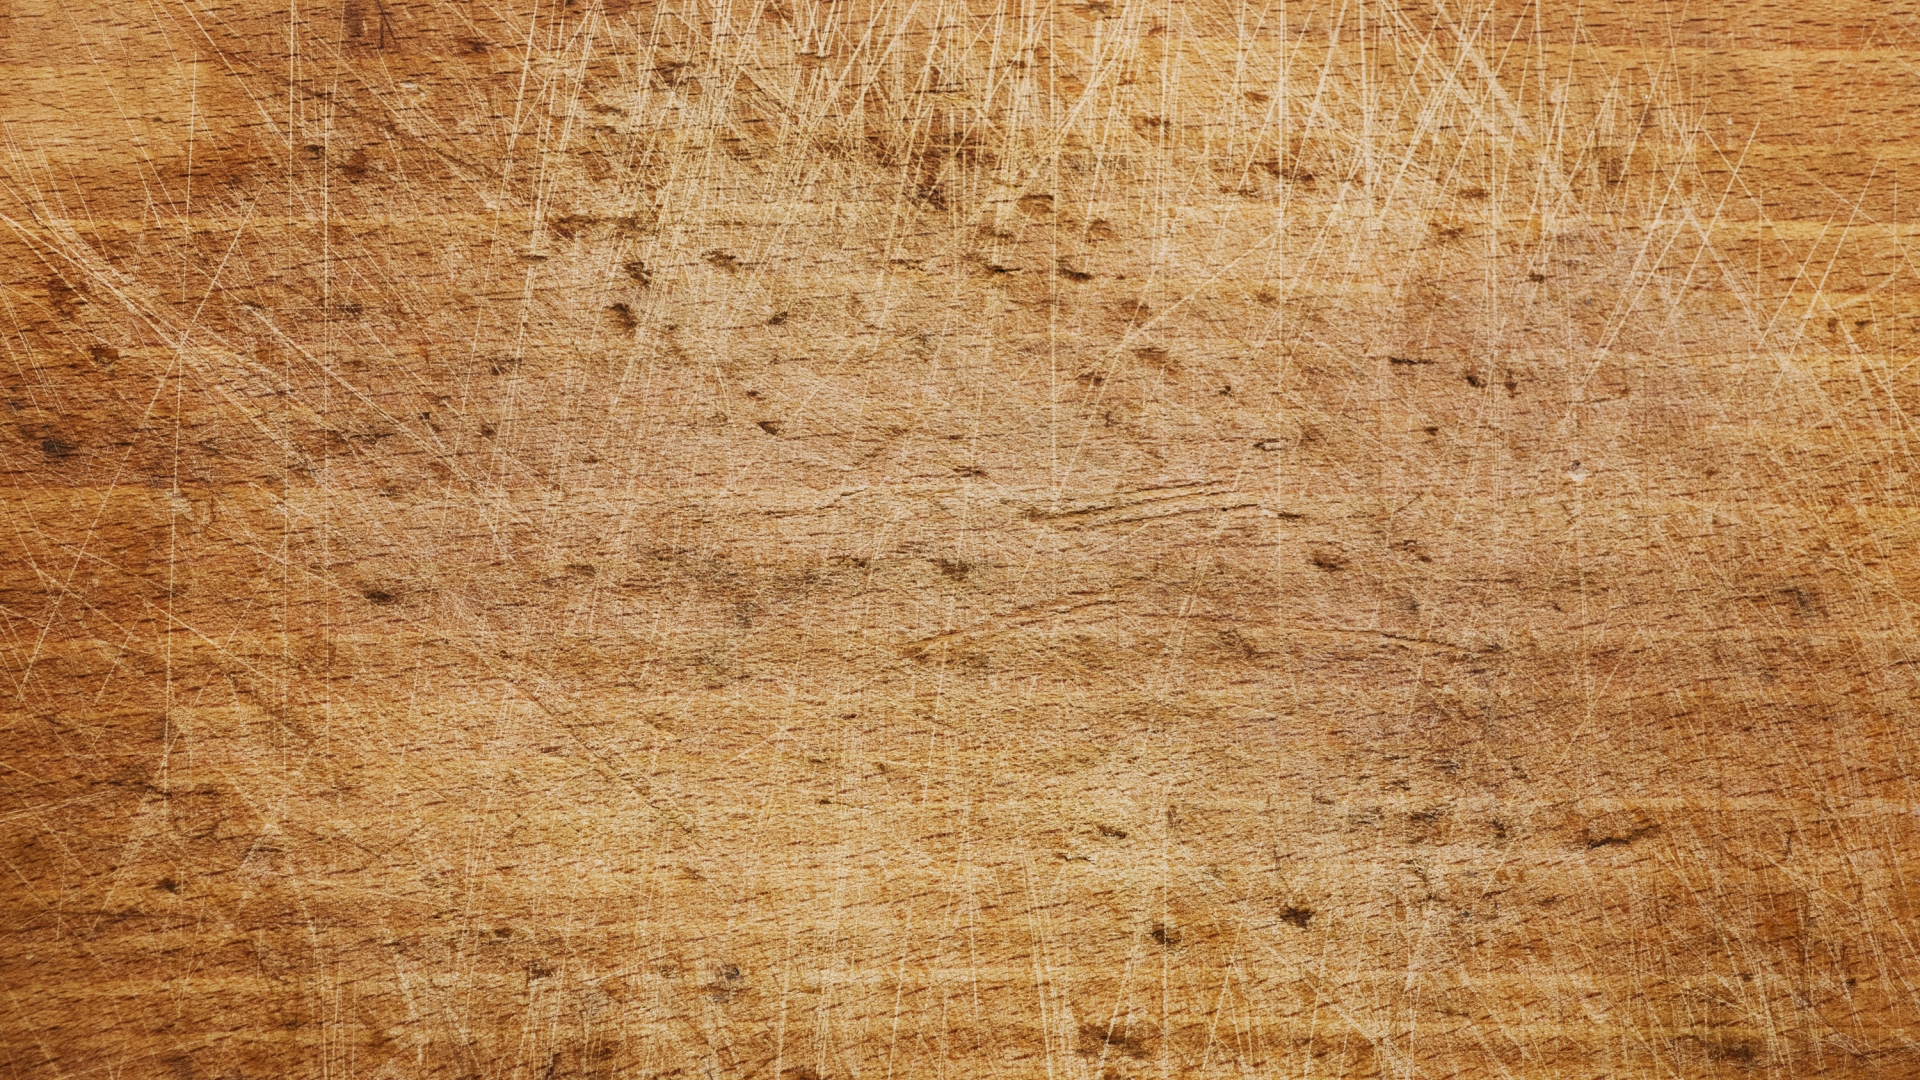
\includegraphics[width=\textwidth]{img/snijplank.jpg}}
\end{center}
\end{comment}

\begin{minipage}[t]{.48\textwidth}
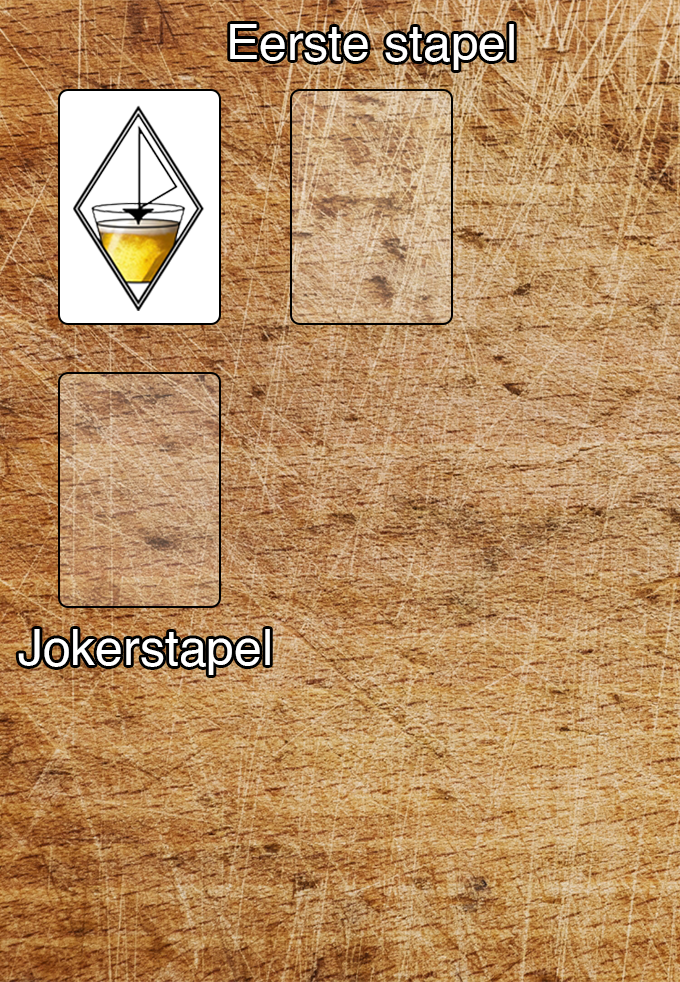
\includegraphics[width=.96\textwidth]{img/Frits_plank_v3.png}
\end{minipage}
\hfill \vrule \hspace{0.35cm}
\begin{minipage}[t]{.48\textwidth}
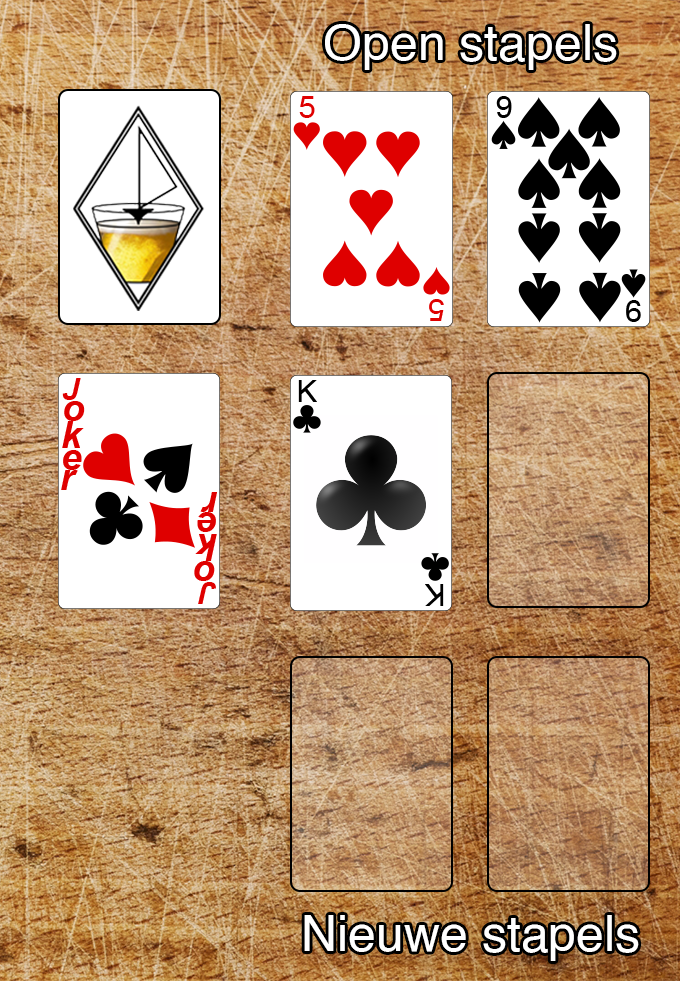
\includegraphics[width=.96\textwidth]{img/Frits_plank_v4_2.png}
\end{minipage}

\vspace{+0.5cm}

\centerline{\Large{\textbf{De volgende pagina beschrijft de zetten}}}